\documentclass[tikz,border=5pt]{standalone}
\usetikzlibrary{arrows.meta}
\usetikzlibrary{backgrounds}
\usetikzlibrary{calc}
\newcommand*{\TickSize}{0.5pt}%

\begin{document}
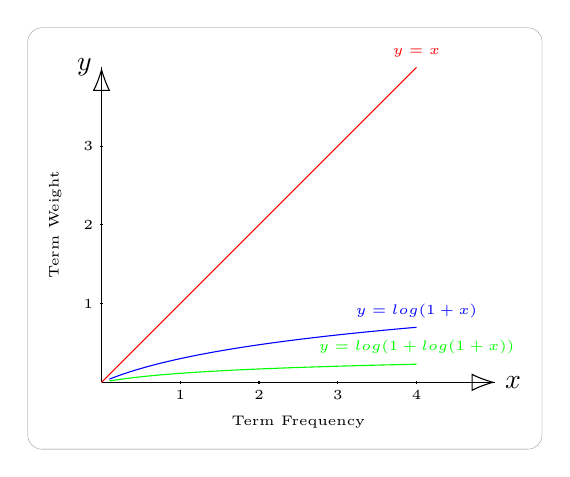
\begin{tikzpicture}
	[framed,background rectangle/.style={ultra thin, rounded corners=5pt, draw=gray}];

	%Axis
	\coordinate (x) at (5,0);
	\coordinate (y) at (0,4);
	\coordinate (o) at (0,0);
	\draw[-{Latex[length=3mm,open]}] (o)--(x) node[right]{$x$};
	\draw (o) -- (x) node [midway, below, sloped, align=center] {\\ \tiny Term Frequency};
	\draw[-{Latex[length=3mm,open]}] (o)--(y) node[left]{$y$};
	\draw (o) -- (y) node [midway, above, sloped, align=center] {\tiny Term Weight \\};

	%coordinate
	\draw [draw=red]plot [domain=0:4] (\x,\x) node[anchor=south,red]{\tiny $y=x$};
	\draw [draw=blue] plot [domain=0.1:4] (\x,{log10(1+\x)}) node[anchor=south,blue]{\tiny$y=log(1+x)$} ;
	\draw [draw=green] plot [domain=0.1:4] (\x,{log10(1+log10(1+\x))}) node[anchor=south,green]{\tiny $y=log(1+log(1+x))$};
	\foreach \x in {1,2,...,4}
	{
    	\draw ($(\x,0) + (0,-\TickSize)$) -- ($(\x,0) + (0,\TickSize)$) node [below] {\tiny $\x$};
    }
	\foreach \y in {1,2,3} 
	{
    	\draw ($(0,\y) + (-\TickSize,0)$) -- ($(0,\y) + (\TickSize,0)$) node [left] {\tiny $\y$};
	}
\end{tikzpicture}
\end{document}